%!TEX root = ../thesis.tex
% ******************************* Thesis Appendix B ********************************

\chapter{Supplementary Tables and Figures}

\ifpdf
    \graphicspath{{Appendix2/Figs/Raster/}{Appendix2/Figs/PDF/}{Appendix2/Figs/}}
\else
    \graphicspath{{Appendix2/Figs/Vector/}{Appendix2/Figs/}}
\fi



\tochide\section{Supplementary Tables for Chapter \ref{chapter:topography}}
\label{sec:aspect-table}

Table \ref{tab:aspect-out} provides additional numerical output from ASPECT. See section \ref{sec:methods-numerical} for definitions of these quantities. Nu is the Nusselt number, the ratio of convective to conductive heat transfer at the surface, calculated as ${\rm Nu} = Y^\prime F^\prime_0 / [k^\prime(T^\prime_1 - T^\prime_0)]$, where $Y^\prime$ is the dimensionless box height, $ F^\prime_0$ is the total surface dimensionless heat flux divided by the dimensionless box width, $k^\prime = 1$ is the dimensionless thermal conductivity, and $T^\prime_1$ and $T^\prime_0$ are the dimensionless temperatures at the bottom and top boundaries respectively.

\begin{table}[h!]
\centering
\caption{Selected time-averaged results of the numerical model. Symbols are defined in the text. \label{tab:aspect-out}}
\footnotesize
\begin{tabular}{@{} c r r r r r r r r r r r @{}}
\toprule
Case & Ra$_1$ & $\Delta \eta$ & Ra$_i$ & $D_{\rm lid}^\prime$ & $\delta_{\rm rh}^\prime$ & $T_i^\prime$ & $T_{\rm lid}^\prime$ & $\Delta T_{\rm rh}^\prime$ & Nu & $h_{\rm rms}^\prime$ & $h_{\rm peak}^\prime$  \\
\midrule

% copy from python
2 & $2 \times 10^{8}$ & $1 \times 10^{6}$ & $7.20 \times 10^{7}$ & $0.133$ & $0.0248$ & $0.926$ & $0.785$ & $0.141$ & $6.17$ & $0.00716$ & $0.0152$ \\
3 & $3 \times 10^{8}$ & $1 \times 10^{6}$ & $1.07 \times 10^{8}$ & $0.118$ & $0.0218$ & $0.925$ & $0.790$ & $0.135$ & $6.97$ & $0.00667$ & $0.0130$ \\
4 & $1 \times 10^{8}$ & $1 \times 10^{7}$ & $3.62 \times 10^{7}$ & $0.199$ & $0.0370$ & $0.937$ & $0.794$ & $0.143$ & $4.10$ & $0.00893$ & $0.0214$ \\
5 & $2 \times 10^{8}$ & $1 \times 10^{7}$ & $7.08 \times 10^{7}$ & $0.165$ & $0.0238$ & $0.936$ & $0.816$ & $0.120$ & $5.12$ & $0.00610$ & $0.0159$ \\
6 & $3 \times 10^{8}$ & $1 \times 10^{7}$ & $1.07 \times 10^{8}$ & $0.148$ & $0.0215$ & $0.936$ & $0.816$ & $0.120$ & $5.70$ & $0.00673$ & $0.0145$ \\
7 & $1 \times 10^{8}$ & $1 \times 10^{8}$ & $3.60 \times 10^{7}$ & $0.235$ & $0.0394$ & $0.945$ & $0.806$ & $0.138$ & $3.50$ & $0.00907$ & $0.0243$ \\
8 & $2 \times 10^{8}$ & $1 \times 10^{8}$ & $7.24 \times 10^{7}$ & $0.199$ & $0.0295$ & $0.945$ & $0.821$ & $0.124$ & $4.23$ & $0.00765$ & $0.0174$ \\
9 & $3 \times 10^{8}$ & $1 \times 10^{8}$ & $1.08 \times 10^{8}$ & $0.179$ & $0.0253$ & $0.945$ & $0.826$ & $0.118$ & $4.75$ & $0.00788$ & $0.0179$ \\
10 & $1 \times 10^{8}$ & $1 \times 10^{9}$ & $3.57 \times 10^{7}$ & $0.274$ & $0.0427$ & $0.950$ & $0.819$ & $0.131$ & $3.03$ & $0.00815$ & $0.0252$ \\
11 & $2 \times 10^{8}$ & $1 \times 10^{9}$ & $7.20 \times 10^{7}$ & $0.232$ & $0.0329$ & $0.951$ & $0.831$ & $0.120$ & $3.65$ & $0.00878$ & $0.0250$ \\
12 & $3 \times 10^{8}$ & $1 \times 10^{9}$ & $1.11 \times 10^{8}$ & $0.213$ & $0.0262$ & $0.952$ & $0.846$ & $0.105$ & $4.07$ & $0.00876$ & $0.0180$ \\





% end copy

\bottomrule
\end{tabular}
\end{table}


\clearpage

\begingroup
%  \makeatletter
%  \setlength{\chapter@bottom@space}{15pt}
%  \makeatother
%\titleformat{\chapter}[display]
%    {\normalfont\huge\bfseries}{\chaptertitlename\ \thechapter}{0pt}{\Huge}
\titlespacing*{\section}{0pt}{20pt}{70pt}  % left, upper, lower
%\let\LaTeXStandardClearpage\clearpage
%\let\clearpage\relax





\tochide\section{Supplementary Figures for Chapter \ref{chapter:rockywater}}
\label{sec:supp-rockywater}


\begin{figure}[!h]
         \centering
         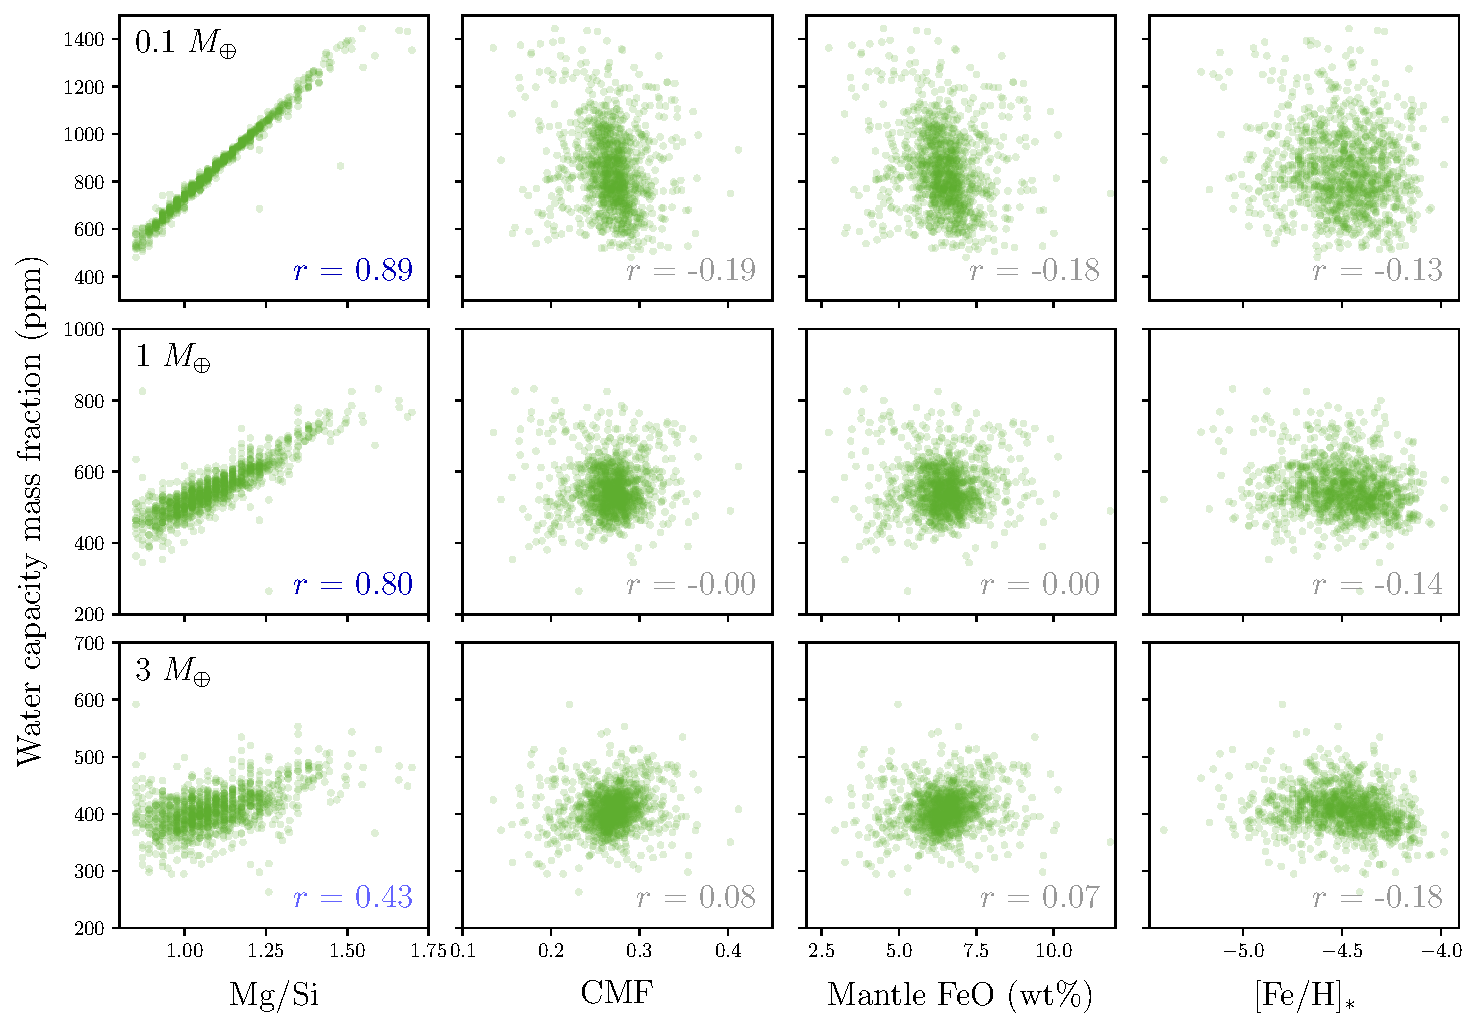
\includegraphics[width=\textwidth]{masses_spread.pdf}
        \caption[Cross plots of mantle water capacity with additional model parameters.]{Cross plots of water capacity (as a fraction of the planet mass), at 0.1 $M_\oplus$ \textit{(top row)}, 0.1 $M_\oplus$ \textit{(middle row)}, and 3 $M_\oplus$ \textit{(bottom row)}, in terms of, from left to right, the molar Mg/Si ratio of the bulk planet, the core mass fraction (CMF), the mantle FeO content in wt\%, and the host star's logarithmic number ratio of Fe to H. The bulk compositions sampled in this figure are based on all planet-hosting stars in the Hypatia Catalog, excepting low Mg/Si compositions for clarity. All planets are simulated with a constant mantle/core molar Fe partitioning of 0.113 and a potential temperature of 1600 K. The value of the Pearson's correlation coefficient $r$ is given in the bottom right corner of each panel. Water capacities correlate significantly only with Mg/Si; there is a high positive correlation for the 0.1 and 1 $M_\oplus$ cases, and a low positive correlation for the 3 $M_\oplus$ cases.}
        \label{fig:wmf_scatter}
\end{figure}


\begin{figure}[!h]
\centering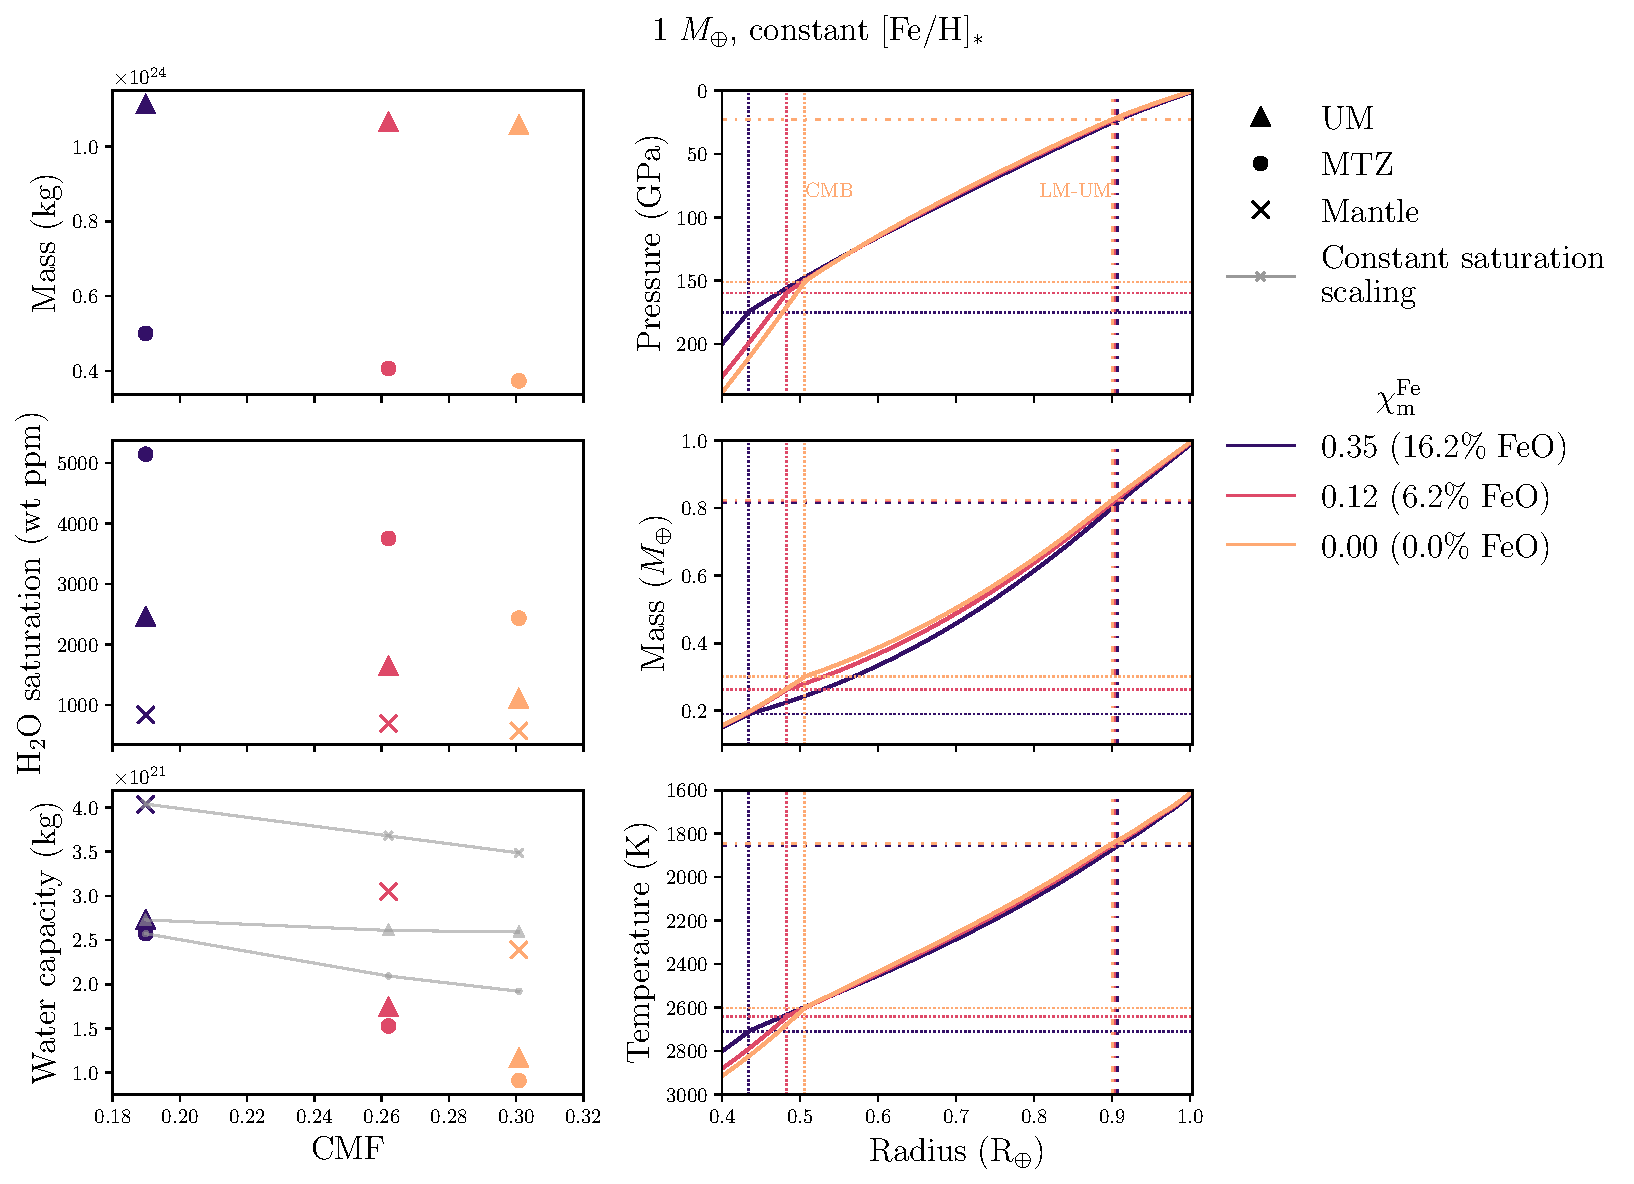
\includegraphics[width=\textwidth]{1M_structure_vs_CMF_coreeff.pdf}
\caption[The effect on mantle water capacity of pressure gradients due to varying the molar fraction of Fe in the mantle.]{The effect on mantle water capacity of pressure gradients due to planet chemistry. Here we fix the host star and planet's bulk abundance of Fe, [Fe/H]$_*$, but vary molar fraction of Fe in the mantle, $\chi^{\rm Fe}_{\rm m}$. The left column shows, from top to bottom, the layer masses, total water concentrations at water saturation with respect to the layer mass, and water capacities, as a function of the resulting core mass fraction (CMF), for the upper mantle (UM; triangles), mantle transition zone (MTZ; circles), and whole mantle (crosses). In the bottom left panel, the grey lines show the water capacities in kg if mineral water saturations were constant (arbitrarily at the value associated with the lowest CMF), and the only factors affecting water capacities were the masses of the layers. The right column shows, from top to bottom, the profiles of pressure, mass, and temperature through the mantle, with vertical and horizontal lines locating the core-mantle boundary (CMB; dotted lines) and the top of the lower mantle (LM-UM; dash-dotted lines). All cases are fixed to a planet mass of 1 $M_\oplus$ and a potential temperature of 1600 K. In the case of variable $\chi^{\rm Fe}_{\rm m}$, moving iron from the core to the mantle has a small positive effect on the mass of the upper mantle, and a larger positive effect on the mineral water saturation contents, which both act to increase the water capacity.}
\label{fig:pressure_gradients_coreeff}
\end{figure}


\begin{figure}
         \centering
         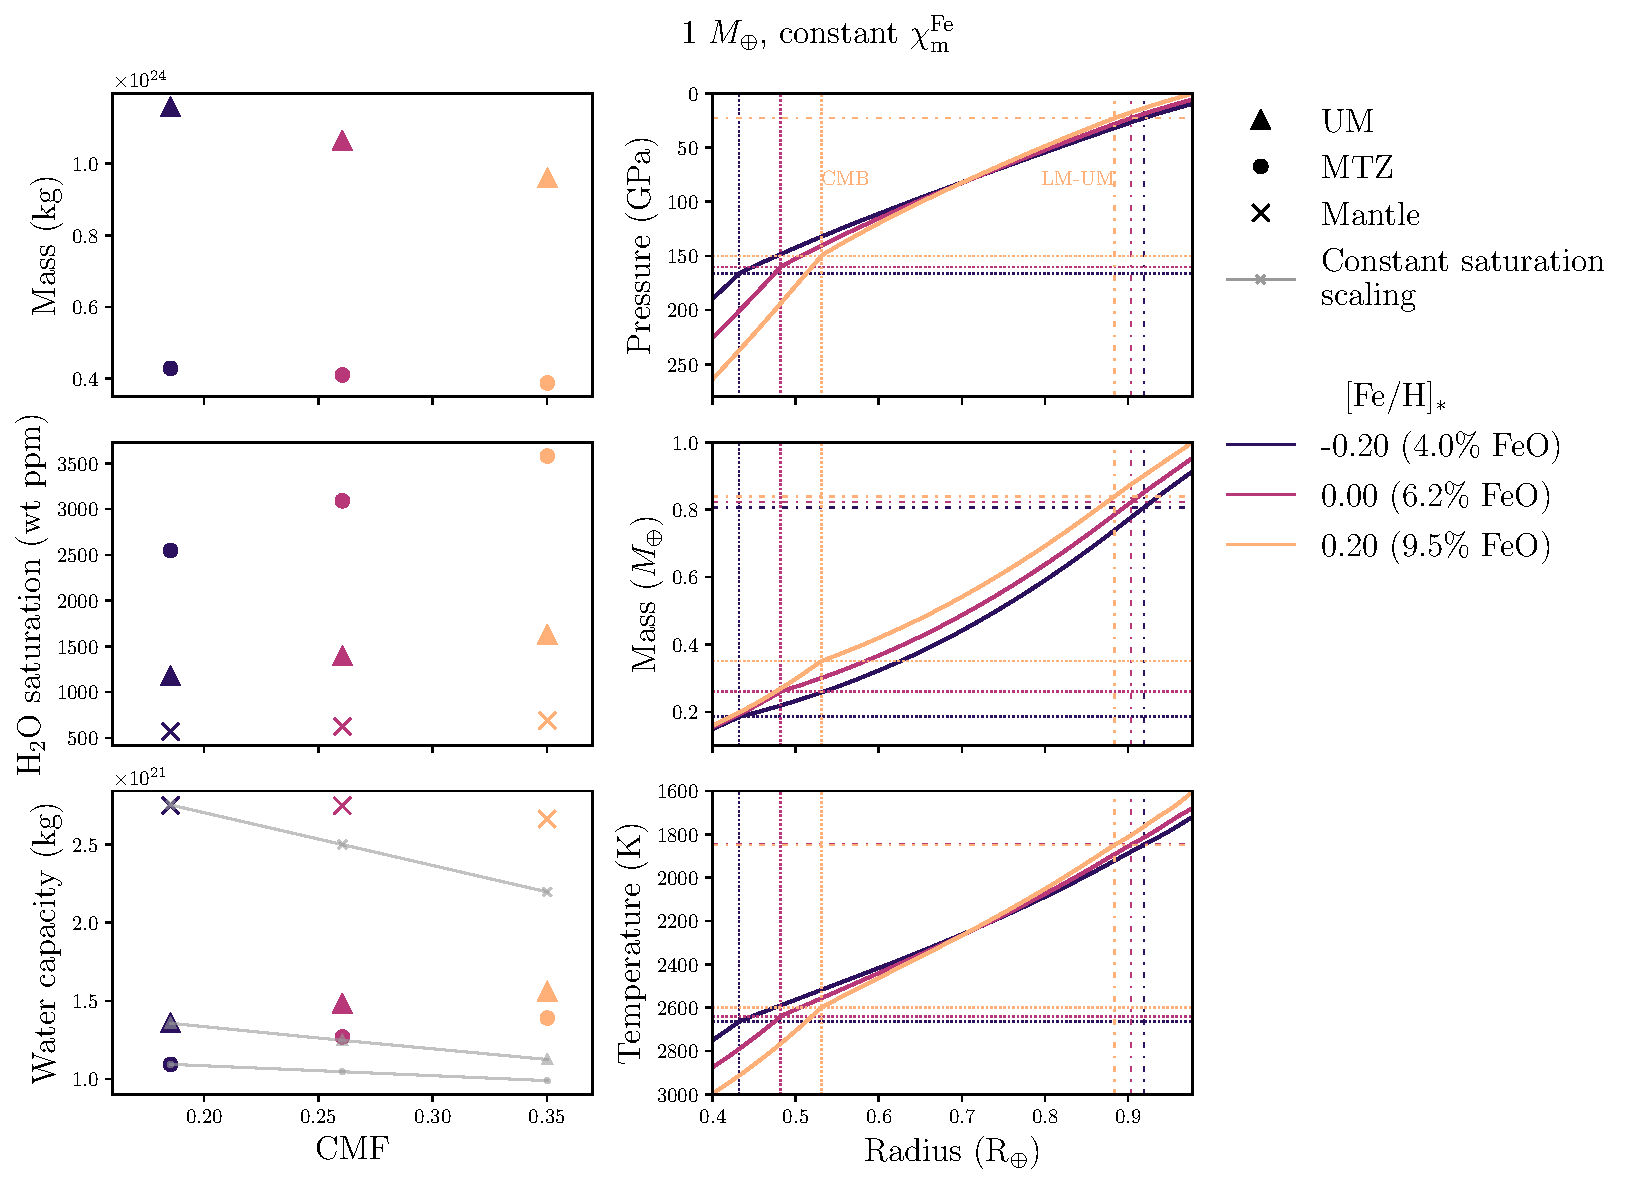
\includegraphics[width=\textwidth]{1M_structure_vs_CMF_feh.pdf}
         \caption[The effect on mantle water capacity of pressure gradients due varying the stellar Fe abundance.]{The same as in Fig. \ref{fig:pressure_gradients_coreeff}, but for a fixed planetary Fe partitioning, $\chi^{\rm Fe}_{\rm m}$, and variable stellar Fe abundance, [Fe/H]$_*$. In the case of variable [Fe/H]$_*$, increasing the overall iron content of the system has a negative effect on the mass of the upper mantle, and a positive effect on the mineral water saturation contents, the results of which nearly cancel out.}
        \label{fig:pressure_gradients_feh}
\end{figure}


\clearpage


\tochide\section{Supplementary Figures for Chapter \ref{chapter:fo2}}
\label{sec:supp-fo2}


\begin{figure}[!htb]
         \centering
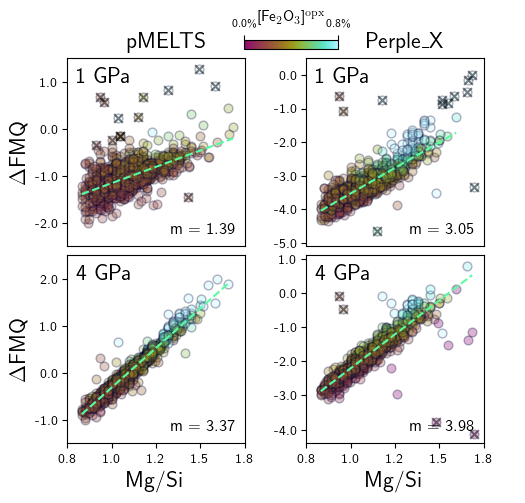
\includegraphics[width=0.8\textwidth]{crossplot_mgsi_fit.png}
        \caption[Linear regression fit of mantle oxygen fugacity with Mg/Si ratio.]{The same cross-plots as the left columns of Figs. \ref{fig:xplots_mlts} and \ref{fig:xplots_px} in the main text but with linear regressions overlain in green: mantle oxygen fugacity, expressed as $\Delta$FMQ, as a function of the mantle molar Mg/Si ratio. Outliers (grey crosses), as determined by their effects on $\chi^2$ using a leave-one-out method, are excluded from the regressions. Slopes $m$ of the regressions are shown in the bottom right corner of each panel. Calculations are performed at $1373\,\text{K}$ and at $1\,{\rm GPa}$ \textit{(top)} and $4\,{\rm GPa}$ \textit{(bottom)}, using pMELTS \textit{(left)} and the \citet{jennings_simple_2015} database in Perple\_X \textit{(right)}. Each point represents a bulk mantle composition estimated from refractory element abundances of planet-hosting stars in the Hypatia Catalog \citep{hinkel_stellar_2014}.\label{fig:mgsi_fit}}
\end{figure}
\begin{figure}[!htb]
         \centering
\bigskip
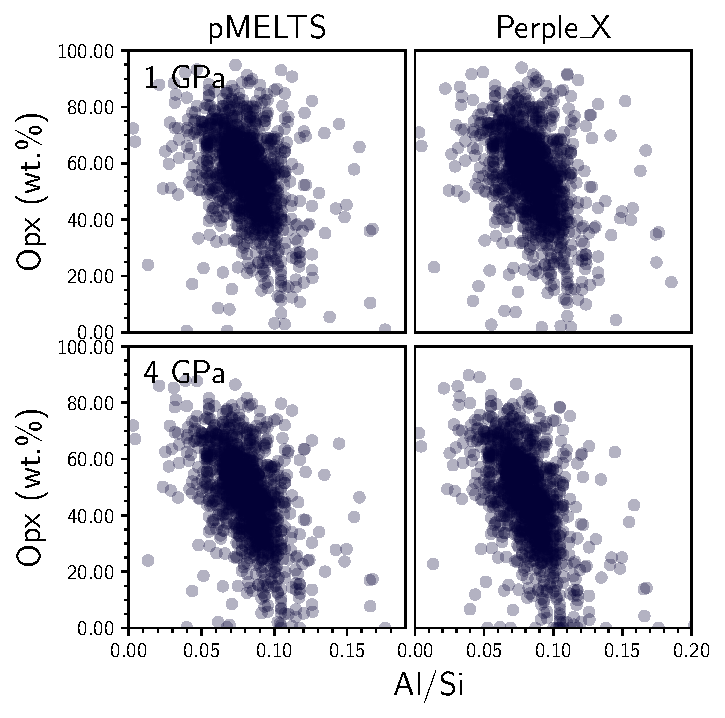
\includegraphics[width=0.7\textwidth]{crossplot_al_opx.pdf}
        \caption[Modality ratios of spinel and garnet to orthopyroxene, as a function of Al/Si.]{Cross plot of the wt.\% modality ratios of an aluminous phase (spinel, Sp, or garnet, Gt) to orthopyroxene (Opx), as a function of the molar Al/Si ratio, estimated for rocky exoplanet mantles and based on refractory element abundances from planet-hosting stars in the Hypatia Catalog \citep{hinkel_stellar_2014}, here assuming an Earth-like molar ratio of core Fe-metal to mantle FeO. Calculations are performed at $1373\,\text{K}$ and at $1\,{\rm GPa}$, nominally the spinel field \textit{(top)}, or $4\,{\rm GPa}$, nominally the garnet field \textit{(bottom)}, using pMELTS \textit{(left)} and the \citet{jennings_simple_2015} database in Perple\_X \textit{(right)}. Note a few extreme cases are not visible in these $y$-axis limits. With increasing Al/Si, higher proportions of the aluminous phase are stabilised at the expense of orthopyroxene.\label{fig:alsi_opx}}
\end{figure}

\endgroup